\section{Theorie}
\label{sec:Theorie}
\subsection{Zielsetzung}
Ziel des Versuchs ist die Überprüfung der Bragg-Bedingung, die Messung des Emissionspektrum für einer Cu-Anode
einer Röntgenröhre und die Bestimmung der Abschirmungskonstanten $\sigma_K$ für verschiedene Materialien durch Messung ihrer Absorptionsspektren.
\subsection{Erzeugung von Röntgenstrahlung}
Röntgenstrahlen können durch die Abbremsung schneller Elektronen erzeugt werden. Dafür wird in einer Röntgenröhre an einer
Glühkathode Elektronen emittiert, die mit einer Spannung im kV Bereich zur Anode hin beschleunigt werden. Beim Auftreffen auf das Anodenmaterial werden 
die Elektronen im Coulombfeld der Atomkerne abgebremst. Die Differenz der kinetischen Energie wird als Photon abgestrahlt. Dieser Teil des Spektrums wird als kontinuierliches 
Bremsspektrum bezeichnet, da jeder beliebige Teil der kinetischen Energie abgegeben werden kann. Der Teil ist in Abbildung \ref{fig:Brems}
\begin{figure}[H]
    \centering
    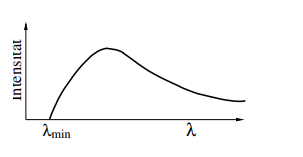
\includegraphics[scale=1.5]{content/Bremsspektrum.png}
    \caption{Bremsspektrum der Röntgenstrahlung \cite{sample}.}
    \label{fig:Brems}
\end{figure}
Die maximale Energie der Photonen kann anhand der minimalen Wellenlänge$\lambda_\text{min}$ abgelesen werden. Diese ergibt sich aus der angelegten Spannung $U$
durch die Formel
\begin{equation}
    \lambda_\text{min}=\frac{h\cdot c}{e_0U}.
    \label{eq:minWelle}
\end{equation}
und beschreibt die Elektronen, die vollständig abgebremst worden sind und somit ihre gesamte kinetische Energie $E_\text{kin}=e_0U$ als Photon mit Energie $E=h\nu$ abgegeben haben.
Zusätzlich wird noch ein für das Anodenmaterial charakteristisches Spektrum. Es entsteht, da die Elektronen das Anodenmaterial ionisieren und dadurch
Elektronen in die innere Schale zurückfallen können. Die Energiedifferenz der Schalen wird als Photon emittiert und ist Teil des Röntgenspektrums.
\subsection{Emissionspektrum}

\subsection{Absorptionsspektrum}
\cite{sample}
